% arara: lualatex: { shell: true }
% arara: latexmk: { clean: partial }
\documentclass[class=book, crop=false, oneside, 12pt]{standalone}
\usepackage{standalone}
\usepackage{../../style}
\usepackage{../../glossary}

\let\isCompiledFromMain\undefined
\usepackage{../../music-tools}

\graphicspath{{./assets/images/}}
\ifdefined\isCompiledFromMain
\else
    \setluaoption{ly}{includepaths}{./assets/scores/}
\fi

\begin{document}

    \chapter{Sheep}

    \section{Introduzione}
    \label{sec:04-intro}

    Sheep è un brano lungo poco più di dieci minuti. 
    durata comparabile a quella delle altri tre canzoni core dell'album

    posizione nel disco
    
    
    come quelle, non è una vera e propria suite, nel senso che non tutti gli elementi della scrittura musicale cambiano, ma solo alcuni. es la tonalità non cambia (o comunque non sempre), nemmeno il bpm. in ultima analisi, pare più una canzone lunga che una suite.

    note di arrangiamento
    genesi e significato
    altre note



    \section{Struttura}
    \label{sec:04-struttura}

    Il brano si può dividere in \emph{quattro} sezioni principali.
    La suddivisione del brano in sezioni si basa su criteri che individuano similitudini intra segmento e differenze extra segmento; in particolare, le caratteristiche principali tenute in considerazione sono dinamica, tonalità e modo, progressione di accordi, voci impiegate e trame melodiche.

    Per comodità consultativa, in questa analisi chiamiamo le quattro sezioni rispettivamente \(\mathcal{A}\), \(\mathcal{B}\), \(\mathcal{C}\) e \(\mathcal{D}\). Il diagramma in Figura~\ref{fig:04-sections-timeline} mostra la posizione dei confini tra le sezioni individuate.

    \begin{figure}[htbp]
        \centering
        \subimport{assets/figures}{sections_timeline.tex}
        \caption[Durata delle varie sezioni del brano.]{Durata delle varie sezioni del brano. In evidenza la struttura del brano: ABCABD.}
        \label{fig:04-sections-timeline}
    \end{figure}

    \begin{figure}[htbp]
        \centering
        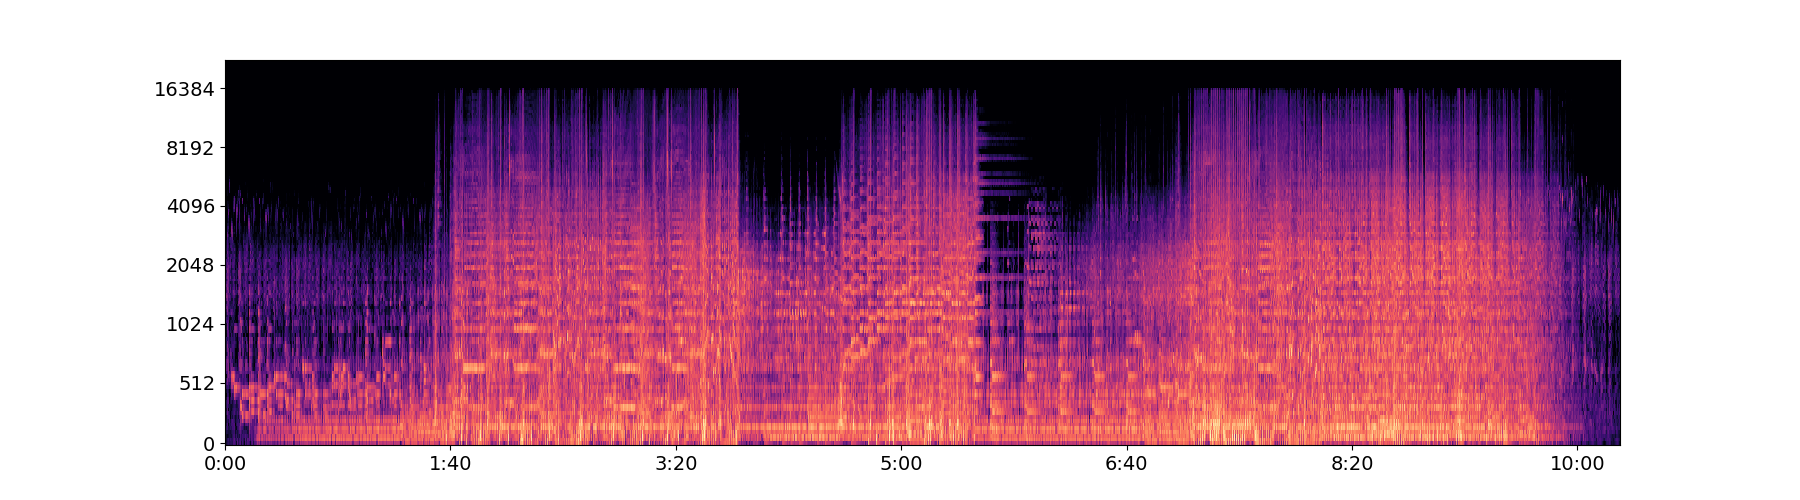
\includegraphics[width=\textwidth]{sheep_spectrogram.png}
        \caption[Spettrogramma rappresentante l'intero brano nel time-frequency domain.]{Spettrogramma rappresentante l'intero brano nel time-frequency domain. Il colore indica l'energia relativa per un momento della canzone in una banda di frequenza. È facile individuare in sezioni piuttosto omogenee dello spettrogramma le sezioni con cui abbiamo descritto il brano già in Fig.\ref{fig:04-sections-timeline}. In particolare, si può notare che  le sezioni \(\mathcal{A}\) e \(\mathcal{C}\) hanno una dinamica molto contenuta, mentre invece le sezioni \(\mathcal{B}\) e \(\mathcal{D}\) sono molto più dense.}
        \label{fig:sheep-spectrogram}
    \end{figure}

    \subsection*{Sezione \(\mathcal{A}\)}
    Sezione di apertura del brano, viene ripresa anche in un secondo momento. È caratterizzata da una dinamica contenuta, che va dal piano al mezzopiano. Dal punto di vista armonico la sezione è prevalentemente occupata da un pedale di D tenuto dal basso; sulla parte conclusiva, in funzione di una modulazione verso la sezione successiva, il pedale viene abbandonato in favore di un movimento verso la sottodominante Am. Lo spazio al di sopra del pedale armonico viene occupato in \(\mathcal{A}1\) dall'iconico assolo di piano elettrico, eseguito con un Rhodes Mk I, mentre in \(\mathcal{A}2\) da una trama armonico/melodica costituita da vari sintetizzatori e campioni di registrazioni ambientali.

    \paragraph{\(\mathcal{A}1\)} 
    Il brano si apre con dei rumori ambientali campionati, nello specifico belati di pecora e cinghuettii di uccelli, cui subito  subentra l'assolo (minuto 0:02). A 0:14 il basso entra in supporto al pedale armonico, con un lento fade in. A 1:20 il cambio di armonia chiama la chiusura dell'assolo. A 1:32 entra la batteria, poco prima dell'inizio della sezione \(\mathcal{B}\).

    \paragraph{\(\mathcal{A}2\)} 
    La ripresa avviene a minuto 5:32. A 6:26 inizia la declamazione del sermone (Sec.\ref{sec:02-animals-lyrics} per dettagli), declamato da una voce processata con vocoder. A minuto 6:48 il il pedale di D viene abbandonato, mentre a 7:02 la batteria rientra.

    \subsection*{Sezione \(\mathcal{B}\)}
    Questa sezione contiene la totalità del testo cantato. La dinamica è molto altra e varia tra il mezzoforte e il forte. Armonicamente si costituisce come ripetizione di due diversi vamp, con sviluppi armonici interessanti. Si ripete circa tre volte: le prime due ripetizioni sono adiacenti e coprono l'intervallo temporale tra 1:42 circa e 3:47, mentre la terza, singola,  inizia a 7:10, dopo la ripresa della sezione \(\mathcal{A}\).

    \subsection*{Sezione \(\mathcal{C}\)}
    Questa sezione è una sorta di ponte tra \(\mathcal{B}\) e la seconda iterazione di \(\mathcal{A}\). Può essere ulteriormente divisa in due sottosezioni: \(\mathcal{C}1\), caratterizzata da una dinamica tra il mezzopiano e il mezzoforte e un pedale di D misolidio, e \(\mathcal{C}2\), caratterizzata invece da una dinamica forte / mezzoforte e da una ripresa finale della sezione \(\mathcal{C}\).

    A 3:46, quando inizia, sono presenti solamente basso, organo e chitarra. A 4:07, si sente un campione  di una registrazione in cui Waters grida \gquotes{stone}, in un feedback loop. A 4:36 il glissato discendente di un synth e l'ingresso della batteria determinano il passaggio a \(\mathcal{C}2\). A 5:18, la ripresa di \(\mathcal{B}\).

    
    \subsection*{Sezione \(\mathcal{D}\)}
    Sezione di chiusura del brano, di cui costituisce a tutti gli effetti una coda. Mantiene la dinamica della precedente sezione ed è caratterizzata da una tensione armonica molto intensa. Inizia circa a minuto 8:06 e si ripete in loop fino al fade out, il quale inizia circa a minuto 9:20. Dopo il minuto 10:00 nessuno strumento è più udibile e restano solo i belati delle pecore, in ripresa dell'inizio del brano.
    
    \section{Tecnica e arrangiamento}
    \label{sec:03-arrangement}

    \subsection{Assolo di Rhodes}

    \begin{sheet}[htbp]
        \centering
        \lilypondfile{./sheep-epiano_solo.ly}
        \caption{Pattern ritmico dell'introduzione.}
        \label{sheet:sheep-epiano_solo}
    \end{sheet}

    \section{Analisi armonica}
    \label{sec:03-harmony}

    \subsection*{Sezione \(\mathcal{A}\)}
    La sezione \(\mathcal{A}\) è caratterizzata nella sua quasi totale interezza da un pedale di D. In \(\mathcal{A}1\) (Rg.\ref{sheet:sheep-a1_chords}), L'assolo di Rhodes fa ampio uso del Si naturale, dando alla sezione una forte impronta modale dorica.     
    
    \begin{sheet}[htbp]
        \centering
        \lilypondfile{./sheep-a1_chords.ly}
        \caption{Progressione di accordi della sezione \(\mathcal{A}1\).}
        \label{sheet:sheep-a1_chords}
    \end{sheet}

    In \(\mathcal{A}2\) (Rg.\ref{sheet:sheep-a2_chords}) il pedale di D viene mantenuto, ma la trama armonica cambia profondamente e al di sopra del pedale viene costruita una fortissima tensione attraverso l'ampio uso dell'accordo di settima diminuita, che viene impiegato dai vari synth e organi, principalmente in forma di arpeggio dei primi e cluster di note dai secondi. In particolare, è interessante notare come il contour armonico venga svelato gradualmente: inizialmente sentiamo un intervallo di terza minore discendente eseguito da un synth in glissando, che ricorda il belato delle pecore.
    Successivamente, un organo interviene con forza, eseguendo un bicordo che introduce per la prima volta il tritono. Infine, un suono ricco di frequenze alte e caratterizzato da un lungo attacco (probabilmente un altro synth, oppure una chitarra suonata in swell) arpeggia l'intero accordo. 
    
    \begin{sheet}[htbp]
        \centering
        \lilypondfile{./sheep-a2_chords.ly}
        \caption{Progressione di accordi della sezione \(\mathcal{A}2\).}
        \label{sheet:sheep-a2_chords}
    \end{sheet}

    Entrambe le varianti si chiudono con una modulazione verso la tonalità di Em, funzionale alla transizione verso la sezione \(\mathcal{B}\). La modulazione è indiretta: viene sfruttato Am, Vm di Re e IVm di Em,  come accordo pivot tra i due centri armonici. Nello specifico, a 24 misure di pedale di D seguono due misure di Am, due di Bm e, infine, altre due misure di Am. Si noti che nessun Em è presente fino all'inizio della sezione successiva; in quest'ottica,  il Bm assume il ruolo di supportare e rendere manifesto il cambio di tonalità, dal momento che è diatonico a Em (Vm) ma non a D dorico. Si noti che in \(\mathcal{A}2\) le ultime \(4\) misure ([ Bm - Bm - Am - Am ]) vengono omesse.

    \subsection*{Sezione \(\mathcal{B}\)}
    La sezione \(\mathcal{B}\) inizia con una semplice progressione in forma [ I - IV - I ], quindi [ Em - C - Em ]. Gli accordi hanno un respiro molto ampio e coprono ciascuno la durata di \(4\) misure e il movimento armonico, che rimbalza tra area tonale di riposo e area di sottodominante, sembrano conferire all'armonia un ruolo di secondo piano, in funzione dell'elemento lirico. La progressione e la frase musicale della voce indicano il Mi come centro armonico; nello specifico, la sezione sembra essere costruita sulla scala di Mi minore naturale.
    Segue un altro vamp di due accordi, ripetuto due volte e composto dagli accordi di [ F\sharp~ - A ], ossia [ II di Em - IV di Em ].  A questi due accordi poi seguono ulteriori \(4\) misure di Em, che concludono il periodo musicale della sezione. L'intera sezione è riportata in Rg.\ref{sheet:sheep-b_chords}

    \begin{sheet}[htbp]
        \centering
        \lilypondfile{./sheep-b_chords.ly}
        \caption{Progressione di accordi della sezione \(\mathcal{B}\).}
        \label{sheet:sheep-b_chords}
    \end{sheet}
    

    Il vamp [ F\sharp~ - A ] è  di difficile contestualizzazione armonica: abbiamo due note non diatoniche nel primio accordo, La\sharp~ e Do\sharp~, e una sola nel secondo, Do\sharp~, in comune con il primo. Di seguito proviamo a valutare alcuni espedienti armonici che potrebbero aiutare a interpretare questo movimento.
    \begin{itemize}
        \item \emph{Interscambio modale}. Il prestito temporaneo di note da scale parallele alla tonica potrebbe spiegare la presenza delle note non diatoniche. Non esiste però nessuna scala che contenga sia F\sharp~, sia A; l'interpretazione di questo passaggio come espressione di interscambio modale appare quindi poco convincente.
        \item \emph{Sostituzione di tritono}. È facile vedere come non si possa usare la sostituzione di tritono per interpretare il vamp: gli accordi sono delle triadi, e la sostituzione di tritono si applica laddove c'è un tritono, presente nella quadriade di un accordo di dominante.
        \item \emph{Dominante Secondaria}. Come sopra, non avendo un vero accordo di dominante, l'interpretazione del passaggio come applicazione di dominanti secondarie appare impropria. Inoltre, anche sorvolando sull'assenza delle settime, non si tratterebbe comunque di una catena di dominanti secondarie: in tal caso ci aspetteremmo di avere [ F\sharp~ - B ], essendo che F\sharp~ è V di B e B è, a sua volta, V di Em.
    \end{itemize}
    
    Proviamo quindi ad adoperare un approccio più descrittivo. Questo vamp è un passaggio carico di tensione, più di qualsiasi altro momento all'interno del brano all'infuori della coda. Questa tensione è data dal passaggio repentino dal Em precedente al F\sharp : i due accordi non hanno alcuna nota in comune, e questo spiazza l'ascoltatore, come se ci si trovasse di fronte a una modulazione indiretta. Il successivo A supporta e tiene alta la tensione creata dall'accordo precedente. In sostanza, a livello macroscopico questo vamp assume il ruolo di momento di massima tensione della sezione; è sopra a questi accordi che il narratore rivela l'inquietudine delle pecore, che percepiscono che c'è qualcosa di sinistro nella società in cui si trovano, ma a cui non riescono a dare né un nome, né un volto. A livello microscopico, l'alternanza tra i due accordi può essere vista come una \emph{mediante cromatica}, ossia una relazione tra un accordo di primo grado, in questo caso F\sharp, e un accordo costruito su un'alterazione della mediante,  in questo caso A, il quale è \flat III di F\sharp~ e diciamo essere mediante cromatica di F\sharp. Una mediante cromatica rinnova l'interesse su un accordo arricchendolo di nuovi colori armonici, mentre ne prolunga la funzione armonica originale \cite[p. 202]{benward2014music}.


    \subsection*{Sezione \(\mathcal{C}\)}

    \subsection*{Sezione \(\mathcal{D}\)}
    La sezione \(\mathcal{D}\) appare inizialmente modale. Il basso e l'organo tengono un pedale di Mi, al di sopra del quale la chitarra esegue un ostinato costruito su una discesa diatonica sul Mi misolidio. Al netto di leggere variazioni sul finale dell'ostinato (si veda Rg.\ref{sheet:sheep-guitar_out_chords}), questo schema viene ripetuto 4 volte, restituendo la ragionevole certezza che l'intera sezione sia un pedale di Mi misolidio. Tuttavia, nella quarta ripetizione dell'ostinato il basso si sposta su un A, spiazzando l'ascoltatore e forzando a ricontestualizzare le trame armoniche precedenti: questo passaggio ha un forte elemento risolutivo, in opposizione alla tensione dominante del precedente E e dovuta al tritono. Questa sezione appare quindi tonale, anzi: può essere vista come una cadenza perfetta ([ V7 - I ]), dove la risoluzione verso il I arriva dopo un periodo di tensione lungo e straziante.

    
    \begin{sheet}[htbp]
        \centering
        \lilypondfile{./sheep-guitar_out_chords.ly}
        \caption{Progressione di accordi della sezione \(\mathcal{D}\). In evidenza gli accordi eseguiti in ostinato dalla chitarra.}
        \label{sheet:sheep-guitar_out_chords}
    \end{sheet}
    

\end{document}